\input{/Users/daniel/github/config/preamble.sty}%This is available at github.com/danimalabares/config
\input{/Users/daniel/github/config/thms-eng.sty}%This is available at github.com/danimalabares/config

\usepackage[style=authortitle-terse,backend=bibtex]{biblatex}
\addbibresource{/Users/daniel/github/config/bibliography.bib}

\begin{document}

\begin{minipage}{\textwidth}
	\begin{minipage}{1\textwidth}
		Geometria Simpl\'etica \hfill Daniel González Casanova Azuela
		
		{\small Profs. Henrique Bursztyn e Leonardo Macarini\hfill\href{https://github.com/danimalabares/sg}{github.com/danimalabares/sg}}
	\end{minipage}
\end{minipage}\vspace{.2cm}\hrule

\vspace{10pt}
{\huge Lista 5}

\tableofcontents

\addcontentsline{toc}{section}{Problem 1}
\begin{thing1}{Problem 1}\leavevmode
	Let  $G$ be a Lie group. Let $X:G\longrightarrow TG$ be a section of the projection $TG\longrightarrow G$, not necessarily smooth. Show that if  $X$ is left invariant (i.e., $dL_g(X)=X\circ L_g$ for all $g\in G$), then $X$ is automatically smooth.

	Conclude that an analogous result holds for differential forms: if a section $\eta:G\to \Lambda^{k}(T^*G)$ is left-invariant ($L^*_g\eta=\eta$), then $\eta$ is a smooth $k$-form. Check that an analogous result holds for $G$-invariant forms on a homogeneous manifold.
\end{thing1}

\begin{proof}[Solution]\leavevmode
	We know that $X_g=dL_g(X_e)$. We want to show that the map $G \to TG:g\mapsto dL_g(X_e)$ is smooth. Suggestion by \href{https://math.stackexchange.com/questions/1126553/left-invariant-vector-fields-smoothness}{Ted Shiffrin at StackExchange} is to consider 
	\begin{align*}
		\mu: G\times G &\longrightarrow G \\
		(g,h) &\longmapsto L_gh=gh
	\end{align*}
	which is smooth and thus has smooth differential which \href{https://math.stackexchange.com/questions/1740179/differential-of-the-multiplication-and-inverse-maps-on-a-lie-group}{turns out to have the expression}
	\begin{align*}
		d\mu: TG\times TG &\longrightarrow TG \\
		(u_g,v_h) &\longmapsto dR_hu_g+dL_g v_h
	\end{align*}
	Choosing $g$ arbitrary, $h=e$, $u_g=0$ and $v_h=X_e$, we obtain
	\[d\mu(u_g,v_h)=dL_gX_e\]
	and, as we have said, this differential depends smoothly on $g$.

	The pullback map is an induced map by $L_g$ on the Grassman algebra:
	\begin{align*}
		L_g^*: \Lambda^{k}(G) &\longrightarrow \Lambda^{k}(G) \\
		\eta &\longmapsto \begin{aligned}
			L_g^*\eta: \mathfrak{X}^k(G) &\longrightarrow \mathbb{R} \\
			(X_1,\ldots,X_k) &\longmapsto \eta(dL_gX_1,\ldots,dL_gX_1)
		\end{aligned}
	\end{align*}
and we have by hypothesis that 
\[L_g^*\eta=\eta.\]

Similarly, group multiplication $\mu$ induces a map on the Grassman algebra:
\begin{align*}
	\mu: \Lambda^{k}(G) \times \Lambda^{k}(G)&\longrightarrow \Lambda^{k}(G) \\
	(\alpha,\beta) &\longmapsto R_h^*\alpha+L_g^*\beta
\end{align*}
so again chosing $\alpha=0$ and $\beta=\eta$ we see that $\eta$ is smooth.

Now let $\eta$ be a $G$-invariant form on a homogeneous manifold $X$. Following \href{https://math.stackexchange.com/questions/4298636/smoothness-of-a-g-invariant-k-form}{Jack Lee's suggestion}, we can pull back $\eta$ to $G$ via the map $\pi:G\to X$, $g\mapsto g\cdot p$ for any fixed $p \in X$. This gives a form $\pi^*\eta$ on $G$ that is left-invariant since  $\eta$ is $G$-invariant: pushing vectors with left-multiplication preserves the orbit of a given point. More explicitly:
\begin{align*}
	L^*_g(\pi^*\eta)&=\pi^*\eta\qquad \text{because}\qquad 
	L^*_g(\pi^*\eta)=\eta\circ d\pi\circ dL_g
\end{align*}
and $\eta$ is constant along vectors on the orbit of $p$, which are the images of $d\pi\circ dL_g$. By the previous exercise we see that $\pi^*\eta$ is smooth.

Then we notice that $\pi$ is a submersion. This follows since $\pi$ is a surjective map (bacuse $X$ is homogeneous)  of constant rank. Constant rank means that $d\pi$ has the same rank at every point of $G$. This can be seen moving around the tangent spaces of both  $G$ and $X$ using the differentials of both the action of  $G$ on $M$, and the left-translation action of $G$ on $G$ as follows. There is a commutative diagram:
\[\begin{tikzcd}
	T_gG\arrow[r,"d\pi"]\arrow[d,swap,"d(\text{action}) "]&T_{gp}X\arrow[d,"d(\text{action})" ]\\
	T_{hg}G\arrow[r,"d\pi"]&T_{hgp}X
\end{tikzcd}\]
and those vertical differentials are diffeomorphisms by smothness of the actions.

Finally we conclude by taking a local inverse $\sigma$ of $\pi$ via inverse function theorem. Then we simply notice that $\eta=\sigma ^*\pi^*\eta$, which is smooth by construction.
\end{proof}

\addcontentsline{toc}{section}{Problem 2}
\begin{thing4}{Problem 2}\leavevmode
	\begin{enumerate}[label=\alph*.]
		\item Prove that any connected Lie group $G$ is generated as a group by any open neighbourhood $U$ of the identity element (i.e. $G=\bigcup_{n=1}^\infty U^n$).
		\item Suppose that two Lie group homomorphisms $\varphi,\psi:G\to H$ are such that $d\varphi|_{e}=d\psi|_{e}$. Show that $\varphi$ and $\psi$ coincide on the connected component of $G$ containing the identity $e$.
	\end{enumerate}
\end{thing4}

\begin{proof}[Solution]\leavevmode
	\begin{enumerate}[label=\alph*.]
		\item Let $U$ be an open  neighbourhood of the identity and define
			\[U^n:=\{g_1\cdot\ldots \cdot g_n:g_{i}\in U\}\]
		for $n \in\mathbb{N}\setminus\{0\}$. We will show that $\bigcup_{n \in\mathbb{N}} U^n$ is a (non-empty, which is trivial since it contains the identity) closed and open set, implying it is $G$ by connectedness.

		We know that for every $g\in G$ right-multiplication $L_g$  is a diffeomorphism of $G$ (because its inverse is $L_{g^{-1}}$). So it is an open map. This means that $U\cdot g$ is open. Now
		\[U^2=U\cdot U=\bigcup_{g\in U}U\cdot g \]
		must be open. Likeways $U^n$ is open and so is $\bigcup_{n \in\mathbb{N}} U^n$.



		\item Let $g\in G$ be any element. Suppose we find a vector $v\in T_eG$ such that its integral curve $\gamma$ passes through $g$ at time $t_0$. Then we can map this vector both by $d\varphi$ and $d\psi$ to obtain a vector $w:=d_e\varphi(v)=d_e\psi(v)\in T_eH$. Then the integral curve $\eta$ of  $w$ is the same as the integral curve of $v$ pushed by either of  $\varphi$ or $\psi$. Let me show this explicitly for self-conviction:
			\begin{quotation}
				$\varphi\circ \gamma(t)=\eta(t)$ for all $t$ because differentaition at $t=0$ yields  $\frac{d}{dt}(\varphi\circ \gamma)\Big|_{t=0}=d_e\varphi\gamma'(0)=d_e\varphi v=\eta'(0)$ so both $\varphi\circ \gamma$ and $\eta$ are solutions to the same differential equation thus coincide.
			\end{quotation}
			Of course the same goes for $\psi$. Then we get that
			\[\gamma(t_0)=g\implies \varphi(g)=\varphi(\gamma(t_0))=\eta(t_0)=\psi(\gamma(t_0))=\psi(g)\]
$\mathsf{OK}$ now we only need to find the vector $v$. The statement is that for every $g\in G$ there is a maximal integral curve starting at the identity passing through $g$. Since $g$ is the same connected component as the identity we can find a curve connecting them. But this curve need not be a maximal integral curve nor homotopic to one. So I'm stuck and I suppose that there is no maximal integral curve. Then all the vectors in the unit ball… \href{https://math.stackexchange.com/questions/1258904/how-to-show-that-for-every-element-g-in-a-lie-group-the-curve-gammat-g}{I'm pretty sure here is the answer}.

	\end{enumerate}
\end{proof}

\addcontentsline{toc}{section}{Problem 3}
\begin{thing1}{Problem 3}\leavevmode
	Consider the Lie groups $\mathsf{SU}(2) =\{A\in\mathcal{M}_{2}(\mathbb{C})|AA^*=\operatorname{Id}, \det A=1\}$ and $\mathsf{SO}(3) =\{A\in\mathcal{M}_{3}(\mathbb{R})|AA^{\mathbf{T}}=\operatorname{Id},\det A=1\}$.
	\begin{enumerate}[label=\alph*.]
		\item Show that
		\[\mathsf{SU}(2) =\left\{ \begin{pmatrix} a&b\\-\bar{b}&\bar{a} \end{pmatrix} ,a,b\in\mathbb{C},|a|^2+|b|^2=1\right\} \]
		Conclude that, as a manifold $\mathsf{SU}(2)$ is diffeomorphic to $S^3$ (hence it is simply connected).

		Recall the definition of the quaternions $\mathbb{H}$. Show that the sphere $S^3$, seen as quaternions of norm 1, inherits a Lie group structure with respect to which it is isomorphic to $\mathsf{SU}(2)$.

	\item Verify that
		\begin{equation}\label{eq:1}
			\mathfrak{su}(2) =\left\{ \begin{pmatrix} i\alpha &\beta\\-\bar{\beta} &-i\alpha \end{pmatrix} ,\alpha\in\mathbb{R},\beta\in\mathbb{C} \right\} .
		\end{equation}
		Consider the identification $\mathfrak{su}(2) \cong \mathbb{R}^{3}$, that takes the element in $\mathfrak{su}(2)$ determined by $\alpha,\beta$ to the vector $(\alpha,\operatorname{Re}\beta,\operatorname{Im}\beta)$ in $\mathbb{R}^{3}$. Observe that, with respect to this identification, $ \det $ in $\mathfrak{su}(2)$ corresponds to $\|\cdot\|^2$ in $\mathbb{R}^{3}$.


	\item Verify that each element $A\in\mathsf{SU}(2)$ defines a linear transformation on the vector space $\mathfrak{su}(2)$ by conjugation: $B\mapsto ABA^{-1}$. Show that, with the identification $\mathfrak{su}(2) \cong \mathbb{R}^{3}$, we obtain a representation (i.e., a linear action) of $\mathsf{SU}(2)$ on $\mathbb{R}^{3}$ that is norm preserving. Conclude that we have homomorphism $\phi:\mathsf{SU}(2) \to \mathsf{O}(3)$, verifying that is image is $\mathsf{SO}(3)$ and its kernel is $\{\operatorname{Id},-\operatorname{Id}\}$.

	\item Conclude that $\mathsf{SU}(2) \cong S^3$ is a double cover of $\mathsf{SO}(3)$ *hence is its universal cover, since it's simply connected), qnd the covering map identifies antipodal points of $S^3$. Hence, as manifolds, $\mathsf{SO}(3)$ is identified with $\mathbb{R}P^{3}$.
	\end{enumerate}
\end{thing1}

\begin{proof}[Solution]\leavevmode
	\begin{enumerate}[label=\alph*.]
		\item It is very easy to see that a matrix 
			\[A:=\begin{pmatrix} a &b\\c & d \end{pmatrix} \in\operatorname{Mat}_{2}(\mathbb{C})\]
			satisfying $A A^*=\operatorname{Id}\iff A^*=A^{-1}$ must be of the form
			\[\begin{pmatrix} a &b\\-\bar{b}&\bar{a} \end{pmatrix} \]
			since $A^*=A^{-1}$ translates to
			\[\begin{pmatrix} \bar{a} &\bar{c}\\\bar{b}&\bar{d} \end{pmatrix} =\begin{pmatrix} d&-b\\-c&a\end{pmatrix} \]
			which yields immediately $\bar{a} =d$ and $c=-\bar{b}$.

			Conversely, if $|a|^2+|b|^2=1$ the matrix \[B:=\begin{pmatrix} a &b\\-\bar{b}&\bar{a} \end{pmatrix}\] has determinant
			 \[\det B=a\bar{a}+b \bar{b}=|a|^2+|b|^2=1 \]
			 and its inverse is
			 \[B^{-1}=\begin{pmatrix} \bar{a}&-b\\\bar{b}&a \end{pmatrix} =B^*.\]


			Having estabilshed this expression for $\mathsf{SU}(2)$, it is clear that it is diffeomorphic to $S^3$ since its parameters $a,b\in\mathbb{C}$, $|a|^2+|b|^2=1$, can be understood as vectors $x\in\mathbb{R}^{4}$ of norm 1.

		The quaternions are the only 4-dimensional real division algebra. This means it is a 4-dimensional real vector space equipped with a (non-commutative) multiplication. They are also equipped with a norm that coincides with euclidean norm. With respect to this norm we define the unit sphere $S^3$. 
		
			To see that $S^3$ is a Lie subgroup we first need to check that it is closed under quaternion product. The easiest way to see that is via quaternion conjugate: if $x=x_1+ix_2+jx_3+kx_4$ is a quaternion, its conjugate is $\bar{x}=x_1-ix_2-jx_3-kx_4$. It may be computed that the norm is given by $|x| =x\bar{x}$. Then we see that if $x,y\in S^3$
			\[|xy\overline{xy}|=|xy\bar{y}\bar{x}| =\Big|x|y| \bar{x}\Big|=1\]
			Then the fact that $S^3$ is a Lie group follows from the fact that the restricition (the multiplication and inverse map) of smooth maps to embedded submanifolds remains smooth (\cite{lee}, prop ?).

			An identification between $S^3\subset \mathbb{H}$ and $\mathsf{SU}(2)$ as expressed above is given by
			\[a+bi+cj+dk\longmapsto \begin{pmatrix} a+bi&c+di\\-c+di&a-bi\end{pmatrix} \]
			Checking that this map is a group isomorphism ammounts to checking that matrix multiplication in $\mathsf{SU}(2)$ is the same as quaternion multiplication 


			\item (Proof from \cite{hall}, prop. 3.24.) We will show that $\mathfrak{su}(3)$ is the space of traceless anti-hermitian matrices and \cref{eq:1} will follow.
				\begin{enumerate}[label=\textbf{Step \arabic*}]
					\item Show that the Lie algebra of a matrix Lie group $G$, defined as the tangent space at identity, is the same as the matrices $X$ such that $ \operatorname{exp}(tX) \in G$ for all $t\in\mathbb{R}$. (Inspired, though the proof is different because his definitions are different, in \cite{hall}, coro. 3.46.)

						\begin{proof}[Proof of Step 1]\leavevmode
							First suppose that $X$ is such that $\operatorname{exp}(tX)\in G$ for all $t\in\mathbb{R}$. Then the curve $\gamma(t)=\operatorname{exp}(tX)$, which is contained in $G$, passes through the identity at $t=0$ with velocity $X$, meaning that $X$ is in the tangent space of the identity element.

							For the converse suppose that $X \in T_{\operatorname{Id}}G$. Our definition of exponential map is to move along the integral curve of $X$, say $\gamma_X$, by 1 unit of time. Then
							\[\operatorname{exp}(tX) =\gamma_{tX}(1)=\gamma_X(t)\in G\]
							by homogenity property.

							%Define a curve $\gamma$ via the exponential map (seen in lectures, also see figure): $\gamma(t)=\operatorname{exp}(tX)$ which is in $G$ by definition of exponential map.
	\begin{figure}[H]		\centering
		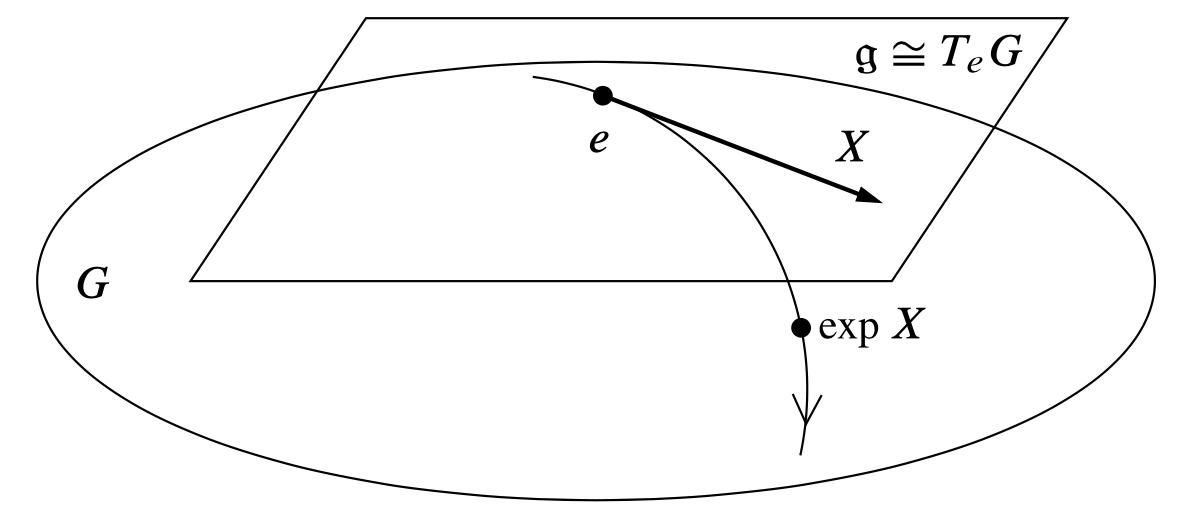
\includegraphics[width=0.4\textwidth]{fig2}	
	\caption*{(I spent way too much time thinking about this…)}\end{figure}

						\end{proof}

					\item Then we look for the matrices such that for all $t\in\mathbb{R}$,
						\[\operatorname{exp}(tX)^* =\operatorname{exp}(tX)^{-1}=\operatorname{exp}(-tX) \qquad \text{ and} \qquad \det \operatorname{exp}(tX)=1. \]
						This means that
						\[\operatorname{exp}(tX^*) =\operatorname{exp}(-tX) \qquad \text{and} \qquad \operatorname{ Tr}(X)=0.\]
						The first implication is the result of the general facts that $(e^{A})^*=e^{A^*}$ and $(e^A)^{-1}=e^{A^{-1}}$. Let's have a look at the second one:
\begin{quotation}
	{\color{3}$(e^A)^{-1}=e^{A^{-1}}$}\hspace{.5em}This is nicely shown in \cite{lee} as follows. For any $X\in\mathsf{Lie}(G)$ map $t\mapsto \operatorname{exp}(tX)$ is a group homomorphism  $\mathbb{R}\to G$ because $\operatorname{exp}((t_1+t_2)X)=\operatorname{exp}(t_1X)\operatorname{exp}(t_2X)$ (but of course that could be justified…) anyway from this it follows that this map preserves inverses, which what we wanted.
\end{quotation}

						Now let's have a look at why determinant 1 in Lie group translates to vanishing trace in Lie algebra.
\begin{quotation}
	{\color{3}\bfseries $\forall X\in\mathcal{M}_{n}(\mathbb{C}), \;\det e^X=e^{\operatorname{tr}X}$.}\hspace{.5em}This is easy to see if $X$ is diagonalizable with eigenvalues  $\lambda_1,\ldots,\lambda_n$; then the eigenvalues of $e^{X}$ are $e^{\lambda_1},\ldots,e^{\lambda_n}$. So $\det e^X=\prod e^{\lambda_i}=e^{\sum \lambda_i}=e^{\operatorname{tr}X}$. But if $X$ is not diagonalizable we must do Jordan decomposition and some more computations.
\end{quotation}

						Finally, differentiating and evaluating at $t=0$ the equation $\operatorname{exp}(tX^*) =\operatorname{exp}(-tX)$ gives $X^*=-X$. (See \cite{hall}, prop. 2.4. It is intuitive but not immediate.)

						In conclusion, we see that
						\[\mathfrak{su}(2)=\{X\in\mathcal{M}_{2\times 2}(\mathbb{C}):X^* =-X\text{ and }\operatorname{Tr}(X)=0 \}\]
		
					\item It is immediate that the right-hand side in \cref{eq:1} is contained in the set above. For the other inclusion first notice that the condition $X^*=-X$ makes the entries in the diagonal be such that
						\begin{align*}							x+iy&=-\overline{x+iy}=-(x-iy)=-x+iy\implies x=-x\implies x=0						\end{align*}
						while the traceless condition implies the two entries in the diagonal must be additive inverses. For the entries in the antidiagonal we literally see the definition of conjugate transpose.
				\end{enumerate}

Now let's identify $\mathfrak{su}(2)$ with $\mathbb{R}^{3}$ via $\alpha,\beta \mapsto (\alpha,\operatorname{Re}\beta,\operatorname{Im}\beta)$. We immediately see that
\[\det \begin{pmatrix} i\alpha&\beta\\-\bar{\beta} &-i\alpha\end{pmatrix} =i\alpha(-i\alpha)=\beta(-\bar{\beta} )=\alpha^2+|\beta|^2=\|(\alpha,\operatorname{Re}\beta,\operatorname{Im}\beta)\|^2\]

\item De acordo com o exercício anterior, é suficiente mostrar que $ABA^{-1}$ tem traço zero e $ABA^{-1}=-(ABA^{-1})^*$. A primeira propriedade é imediata dado que, em geral, $\operatorname{Tr}(XY)=\operatorname{Tr}(YX)$. Para a segunda propriedade note que
	\[(ABA^{-1})^*=(A^{-1})^*B^*A^*=(A^*)^*(-B)A^{-1}=-ABA^{-1}\]
	O fato de que essa ação em $\mathsf{SU}(2)$ preserva a norma é immediato do item anterior e do fato de que determinante de um produto de matrizes é o produto dos determinantes.

	Isso significa que cada elemento em $\mathsf{SU}(2)$ age como uma isometria linear $\mathbb{R}^{3}\to \mathbb{R}^{3}$, i.e. temos um mapa 
	\begin{align*}
	\varphi:\mathsf{SU}(2) &\longrightarrow \mathsf{O}(3) \\
	A &\longmapsto I_A
\end{align*}
onde
\begin{align*}
	I_A: \mathfrak{su}(2) \cong \mathbb{R}^{3} &\longrightarrow \mathfrak{su}(2) \cong \mathbb{R}^{3} \\
		B &\longmapsto ABA^{-1}
\end{align*}

	$\varphi$ é um homomorfismo já que para $A,A'\in  \mathsf{SU}(2)$ e $B\in\mathfrak{su}(2)$ temos que
	\[I_{A A'}B=(A A')B(A A')^{-1}=A\Big(A'B(A')^{-1}\Big)A^{-1}=(I_A \circ  I_{A'})B.\]
	Para determinar que matriz corresponde com a transformação $I_A$ mediante a identificação $\mathfrak{su}(2) \cong \mathbb{R}^{3}$, suponha que
	\[A=\begin{pmatrix} a&b\\-\bar{b}&\bar{a} \end{pmatrix}, \qquad B=\begin{pmatrix} i\alpha &\beta\\-\overline{\beta} &-i\alpha\end{pmatrix}  \]
	Daí,
\begin{align*}
	ABA^{-1}&=ABA^*=\begin{pmatrix} a&b\\-\bar{b}&\bar{a} \end{pmatrix}\begin{pmatrix} i\alpha &\beta\\-\overline{\beta}&-i\alpha \end{pmatrix}\begin{pmatrix} \overline{a}&-b\\\bar{b}&a \end{pmatrix} \\
&=\begin{pmatrix} a&b\\-\bar{b}&\bar{a} \end{pmatrix}\begin{pmatrix} i \alpha\overline{a}+\beta\overline{b} & -i\alpha b + \beta a\\ -\overline{\beta}\overline{a}-i\alpha \overline{b} & \overline{\beta}b-i \alpha a \end{pmatrix}\\
&=\begin{pmatrix} a(i \alpha \overline{a}+\beta\overline{b})+b(-\overline{\beta}\overline{a}-i\alpha\overline{b}) &  a(-i \alpha b+\beta a)+b(\overline{\beta}b-i\alpha a)\\ * & * \end{pmatrix} 
\end{align*}
Daí, se $(x_1,x_2,x_3)$ é vetor correspondente a $ABA^{-1}$, vemos que
\begin{align*}
	ix_1&=a(i \alpha \overline{a}+\beta\overline{b})+b(-\overline{\beta}\overline{a}-i\alpha\overline{b}) \\
	&=i|a|^2\alpha+a\overline{b}\beta-b\overline{a}\overline{\beta}-i\alpha|b|^2\\
	x_2+ix_3&=a(-i \alpha b+\beta a)+b(\overline{\beta}b-i\alpha a)\\
	&=-iab \alpha
\end{align*}
Agora considere a base de $\mathfrak{su}(2)$ dada por
\[\begin{pmatrix} i&0\\0&-i \end{pmatrix},\quad \begin{pmatrix} 0&1\\-1&0 \end{pmatrix} ,\quad \begin{pmatrix} 0&i\\-i&0 \end{pmatrix}  \]
que corresponde à base canônica de $\mathbb{R}^{3}$. A matriz da transformação $I_A$  terá nas columnas os vetores correspondentes às imagens dessas treis matrizes. Ussando as formulas anteriores, concluimos que
\[I_A=\begin{pmatrix} |a|^2-|b|^2 & \operatorname{Re}(-i(a\overline{b}-b \overline{a}))& \operatorname{Re}(a \overline{b}+b \overline{a})\\
0 & \operatorname{Re}(a^2+b^2)& \operatorname{Re}(i(a^2-b^2)) \\
-2ab& \operatorname{Im}(a^2+b^2)&\operatorname{Im}(i(a^2-b^2))\end{pmatrix} \]
\end{enumerate}
Para calcular o kernel de $\varphi$ suponha que a matriz anterior é a identidade. Segue que
\begin{align*}
	&=
\end{align*}

\item Supondo que mostramos que a imagem de $\varphi$ é $\mathsf{SO}(3)$ com kernel $\{\operatorname{Id},-\operatorname{Id}\}$, temos o isomorfismo
	\[\dfrac{\mathsf{SU}(2)}{\{\operatorname{Id},-\operatorname{Id}\}}\cong \mathsf{SO}(3)\]
Suponha que dois elementos $A,B \in\mathsf{SU}(2)$ estão na mesma classe de equivâlencia no quociente. Então
\[AB^{-1}\in\{\operatorname{Id},-\operatorname{Id}\}\iff A=B \text{ ou }A=-B \]
Assim, cada elemento de $\mathsf{SO}(3)$ correponde com dois elementos de $\mathsf{SU}(2)$. Como $\{\operatorname{Id},-\operatorname{Id}\}$ age de maneira prórpia, livre e disonctínua em $\mathsf{SU}(2)$, temos um recobrimento de $\mathsf{SO}(3)$. Também é claro que estamos identificando pontos antípodas de $S^3$ já que ser antípoda em $S^3$ corresponde com o produto com $-\operatorname{Id}$. Note que $\mathbb{R}P^{3}\cong S^3/\mathbb{Z}_2$.
	de modo que $\mathsf{SU}(2)$ é um recobrimento de $\mathsf{SO}(3)$: cada ponto de $\mathsf{SO}(3)$ tem uma preimagem composta por dois elementos
\end{proof}

\addcontentsline{toc}{section}{Problem 4}
\begin{thing4}{Problem 4}\leavevmode
	Let $\mathfrak{g}$ be the Lie algebra of a Lie group $G$, and let  $k:\mathfrak{g} \times \mathfrak{g}\to \mathbb{R}$be a symmetric bilinear form that is $\operatorname{Ad}$-invariant (i.e. $k(\operatorname{Ad}_g(u),\operatorname{Ad}_g(v))=k(u,v)$ for $g\in G$).
	\begin{enumerate}[label=\alph*.]
		\item Show that the map
			\begin{equation}\label{Eq:4a}\begin{aligned}
				k^\sharp:\mathfrak{g}  &\longrightarrow \mathfrak{g}^* \\
				k^\sharp(u)(v) &=k(u,v)\end{aligned}
			\end{equation}
			is $G$-equivariant:
			\[k^\sharp \circ \operatorname{Ad}_g=(\operatorname{Ad}^*)_g\circ k^\sharp,\qquad \forall g\in G\]
			[\textit{Recall:} $(\operatorname{Ad}^* )_g:=(\operatorname{Ad}_{g^{-1}})^*$.] In particular, when $k$ is nondegenerate (i.e. $k^\sharp$ is an isomorphism), the adjoint and coadjoint actions are equivalent.

		\item Verify that \cref{Eq:4a} implies that $k([w,u],v)=-k(u,[w,v])$,  $\forall u,v,w\in\mathfrak{g}$, and that both conditions are equivalent when $G$ is connected.
	\end{enumerate}
\end{thing4}

\begin{proof}[Solução]
	\begin{enumerate}[label=\alph*.]
		\item É só abrir as definições . Fixe um elemento $x\in\mathfrak{g}$. No lado esquerdo, temos
			\[\Big(k^\sharp \circ \operatorname{Ad}_g\Big)(x)=k^\sharp(\operatorname{Ad}_gx)=k(\operatorname{Ad}_gx,\cdot )\]
			e no lado direito,
			\[\Big((\operatorname{Ad}^* )_g\circ k^\sharp \Big) (x)=\operatorname{Ad}^*_g(k^\sharp (x))=\operatorname{Ad}^* _g(k(x,\cdot ))=k(x,\operatorname{Ad}_{g^{-1}}\cdot )\]
			mas, como $k$ é $\operatorname{Ad}$-invariante,
			$k(x,\operatorname{Ad}_{g^{-1}}\cdot )=k(\operatorname{Ad}_gx,\cdot )$.

		\item Must check this later…
	\end{enumerate}
\end{proof}

\addcontentsline{toc}{section}{Problem 5}
\begin{thing1}{Problem 5}\leavevmode
For a Lie algebra $\mathfrak{g}$, there is always a canonical bilinear form $k:\mathfrak{g} \times \mathfrak{g} \to \mathbb{R}$, called \textit{\textbf{Killing form}}, given by:
\[k(u,v)=\operatorname{tr}(\operatorname{ad}_u\operatorname{ad}_v).\]
(\textit{Recall:} $\operatorname{ad}_u:\mathfrak{g} \to \mathfrak{g}$, $\operatorname{ad}_u(v)=[u,v]$.)
\begin{enumerate}[label=\alph*.]
	\item Note that $k$ is symmetric, and check that it is  $\operatorname{Ad}$-invariant.
	\item A Lie algebra is called \textit{\textbf{semi-simple}} if $k$ is nondegenerate. Show that $\mathfrak{so}(3)$ is semi-simple.
\end{enumerate}
\end{thing1}

\begin{proof}[Solution]\leavevmode
	\begin{enumerate}[label=\alph*.]
		\item O fato de $k$ ser simétrica segue de que, em geral, $\operatorname{tr}(AB)=\operatorname{tr}(BA)$. Para ver que $k$ é $\operatorname{Ad}$-invariante vamos mostrar que (a idea vem de \href{https://math.stackexchange.com/questions/2409279/showing-killing-form-is-ad-invariant}{StackExchange}):
	\begin{equation}\label{Eq:2}	\operatorname{ad}_{\operatorname{Ad}_gu}=\operatorname{Ad}_g\circ \operatorname{ad}_u\circ \operatorname{Ad}_{g^{-1}}.
		\end{equation}
			Supondo isso, é fácil ver que
			\begin{align*}
				\operatorname{ad}_{\operatorname{Ad}_gu}\circ \operatorname{ad}_{\operatorname{Ad}_{g}v}&=\operatorname{Ad}_{g}\circ \operatorname{ad}_u\circ \operatorname{Ad}_{g^{-1}}\circ \operatorname{Ad}_g\circ \operatorname{ad}_v\circ \operatorname{Ad}_{g^{-1}}\\
				&=\operatorname{Ad}_g\circ \operatorname{ad}_u\circ \operatorname{ad}_v\circ \operatorname{Ad}_{g^{-1}}
			\end{align*}
			e o resultado segue do fato de que a traça é invariante baixo mudanças de coordenadas e que $\operatorname{Ad}_g^{-1}=\operatorname{Ad}_{g^{-1}}$. Isso último segue de que o mapa inverso de $I_g$  é $I_{g^{-1}}$, assim as derivadas deles também são inversa uma da outra.

			Agora vamos mostrar \cref{Eq:2}. Pegue $x\in\mathfrak{g}$. O lado esquerdo diz que
			\[\operatorname{ad}_{\operatorname{Ad}_gu}x=[\operatorname{Ad}_gu,x]\]
			enquanto o direito diz que
			\[\Big(\operatorname{Ad}_g\circ \operatorname{ad}_u\circ \operatorname{Ad}_{g^{-1}}\Big)x=\operatorname{Ad}_g[u,\operatorname{Ad}_{g^{-1}}x]=[\operatorname{Ad}_gu,x\]
			já que $\operatorname{Ad}_g=d_eI_g$ não é apenas um automorfismo linear, mas é um automorfismo de álgebra de Lie, i.e. $\operatorname{Ad}_g[x,y]=[\operatorname{Ad}_gx,\operatorname{Ad}_gy]$ para $x,y\in\mathfrak{g}$. Isso segue do fato de que o pushforward de colchete de Lie de dois campos vetoriais e o colchete dos pushforwards dos campos vetoriais (ver \cite{lee}, coro. 8.31).
		
\item 
	\end{enumerate}
\end{proof}

\addcontentsline{toc}{section}{Problem 6}
\begin{thing4}{Problem 6}\leavevmode
	Consider the linear isomorphism $\mathbb{R}^{3}\to \mathfrak{so}(3)$, given by
	\[v=(x,y,z)\longmapsto \hat{v}:=\begin{pmatrix} 0&-z&y\\z&0&-x\\-y&x&0 \end{pmatrix} \]
	\begin{enumerate}[label=\alph*.]
		\item Describe the Lie bracket on $\mathbb{R}^{3}$ induced by the commutator in $\mathfrak{so}(3)$, and the inner product in $\mathfrak{so}(3)$ that corresponds to the canonical inner product in $\mathbb{R}^{3}$.

		\item Describe the $\mathsf{SO}(3)$-action on $\mathbb{R}^{3}$ corresponding to the adjoint action, its orbits, as well as its infinitesimal generators. Find (without any calculation!) a description of the coadjoint action on $\mathbb{R}^{3}$ (identified with $(\mathbb{R}^{3})^*$ through the canonical inner product).
	\end{enumerate}
\end{thing4}

\begin{proof}[Solution]\leavevmode
	\begin{enumerate}[label=\alph*.]
		\item Lembre que
			\[\mathsf{SO}(3) =\{A\in\mathcal{M}_{3}(\mathbb{R}):A A^{\mathbf{T}}=\operatorname{Id},\det A=1\}\]
			\[\mathfrak{so}(3) =\{A\in\mathcal{M}_{3}(\mathbb{R}):A=-A^{\mathbf{T}}\}\]
Isso explica por que as matrizes em $\mathfrak{so}(3)$ tem a forma mostrada acima. O isomorfismo com $\mathbb{R}^{3}$ é dado por
	\begin{align*}
		 \mathfrak{so}(3) &\longrightarrow \mathbb{R}^{3} \\
		\begin{pmatrix} 0&-z&y\\z&0&-x\\-y&x&0 \end{pmatrix}  &\longmapsto \begin{pmatrix} x\\y\\z \end{pmatrix} =u\\
		[U,V ]& \longmapsto u\times v\\
		\frac{1}{2}\operatorname{tr}(UV^{\mathbf{T}})&\longmapsto\left<u,v\right> 
	\end{align*}
Para comprovar que de fato o commutador de $\mathfrak{so}(3)$ corresponde com o produto vetorial em $\mathbb{R}^{3}$, considere duas matrizes $U,V\in\mathfrak{so}(3)$ e os vetores correspondentes $u=(u_1,u_2,u_3)$, $v=(v_1,v_2,v_3)$. O commutador é
\begin{align*}
	[U,V]=UV-VU&=\begin{pmatrix} 0&-u_3&u_2\\u_3&0&-u_1\\-u_2&u_1&0 \end{pmatrix} \begin{pmatrix} 0&-v_3&v_2\\v_3&0&-v_1\\-v_2&v_1&0 \end{pmatrix} \\
	&- \begin{pmatrix} 0&-v_3&v_2\\v_3&0&-v_1\\-v_2&v_1&0 \end{pmatrix} 
\begin{pmatrix} 0&-u_3&u_2\\u_3&0&-u_1\\-u_2&u_1&0 \end{pmatrix}\end{align*}
	\end{enumerate}
	a entrada $(3,2)$ da matriz resultante  é a primeira coordenada do vetor correspondente a $[U,V]$; esse numero é claramente $u_1v_3-u_3v_2$. Analogamente, a segunda coordenada é $u_3v_1-u_1v_3$, enquanto a terceira $u_1v_2-u_2v_1$. Essas são as coordenadas de $u\times v$.

Para ver que o produto interno de $\mathbb{R}^{3}$ corresponde com $\frac{1}{2}\operatorname{tr}$ note que
\begin{align*}
	UV^{\mathbf{T}}=U(-V)&=\begin{pmatrix} 0&-u_3&u_2\\u_3&0&-u_1\\-u_2&u_1&0 \end{pmatrix} \begin{pmatrix} 0&v_3&-v_2\\-v_3&0&v_1\\v_2&-v_1&0 \end{pmatrix} \\
		       &=\begin{pmatrix} u_3v_3+u_2v_2&*&*\\ *&u_3v_3+u_1v_1&*\\ *&*&u_2v_2+u_1v_1 \end{pmatrix} 
\end{align*}

\item Agora vamos calcular a ação adjunta. 
Primeiro notemos que a ação adjunta, definida como a derivada do operador $I_A(X)=AXA^{-1}$, é ela mesma. Talvez esse é um fato obvio porque $I_A$  é um mapa linear, e a sua derivada coincide com ele. Porém, tem um argumento mais explícito no \href{https://math.stackexchange.com/questions/512026/prove-that-the-action-of-a-lie-group-on-its-lie-algebra-via-the-adjoint-represen}{StackExchange}: a ação adjunta em um vetor  $X\in\mathfrak{so}(3)$ que seja a derivada em $t=0$ da curva $\gamma\subset \mathsf{SO}(3)$, i.e.  $\gamma'(0)=X$, é simplesmente $\frac{d}{dt}A\gamma(t)A^{-1}\Big|_{t=0}=AXA^{-1}$. A observação chave é que como a álgebra de Lie $\mathfrak{so}(3)$ é um álgebra de matrizes, o produto do lado direito está bem definido.

Em fim, agora vou seguir \href{https://www.ethaneade.org/lie.pdf}{este documento} para achar uma matriz que representa esse operador linear quando identificamos $\mathfrak{so}(3)$ com $\mathbb{R}^{3}$. Mais precisamente, queremos achar uma matriz  $\overline{\operatorname{Ad}_A}$ tal que $\operatorname{Ad}_AX=AXA^{-1}\rightsquigarrow \overline{\operatorname{Ad}_A}x$ onde $x\in\mathbb{R}^{3}$  representa a matriz $X\in\mathfrak{so}(3)$. Vamos ver que de fato essa matriz é $A$.

O truque é usar que as matrizes em $\mathsf{SO}(3)$, sendo isometrías de $\mathbb{R}^{3}$, preservam o produto vetorial, i.e. $Ax\times Ay=A(x \times y)$ para qualquer $x,y\in\mathbb{R}^{3}$.
\begin{align*}
	\operatorname{Ad}_AXAy&=
\end{align*}
\end{proof}

\addcontentsline{toc}{section}{Problem 7}
\begin{thing1}{Problem 7}\leavevmode
	Let $(V,\Omega)$ be a symplectic vector space, and consider $H:=V\times \mathbb{R}=\{(v,t)\}$. This space $H$ with the multiplication
	\[(v_1,t_1)\cdot(v_2,t_2)=\left( v_1+v_2,\frac{1}{2}\Omega(v_1,v_2)+t_1+t_2 \right) \]
	is a Lie group called the \textit{\textbf{Heisenberg group}} (find the identity elements and inverses in  $H$).
	\begin{enumerate}[label=\alph*.]
		\item Show (directly from the conjugation formula in $H$) that $\operatorname{Ad}_{(v,t)}(X,r)=(X,r+\Omega(v,X))$, for $(X,r)\in\mathfrak{h}=\mathsf{Lie}(H) =V\times \mathbb{R}$. Describe the adjoint orbits, verifying that their possible dimensions are zero and one.
		\item Verify that $\operatorname{ad}_{(Y,s)}(X,r)=(0,\Omega(Y,X))$. [Recalling that $\operatorname{ad}_{(Y,s)}(X,r)=[(Y,s),(X,r)]$, we obtain a formula for the Lie bracket in $ \mathfrak{h}$.]
		\item Describe the coadjoint action of $H$ on $\mathfrak{h}^*=V^*\times \mathbb{R}^*$ and its orbits, analyzing the possible dimensions.
	\end{enumerate}
\end{thing1}

\begin{proof}[Solution]\leavevmode
É imediato que a identidade em $H$ é $(0,0)\in V\times \mathbb{R}$, e o elemento inverso de $(v,t)$  é $(-v,-t)$.
 \begin{enumerate}[label=\alph*.]
	\item Primeiro note que $\operatorname{Ad}_{(v,t)}X=(v,t)\cdot X\cdot(-v,-t)$ onde $\cdot$ denota o produto en $H\cong \mathfrak{h}$ (esse isomorfismo é claro já que $H$ é um espaço vetorial, assim o espaço tangente em $(0,0)$  é isomofo a ele). Para justificar isso (como no exercício anterior), considere uma curva $\gamma\subset H$ tal que $\gamma(0)=(0,0)$ e $\gamma'(0)=(X,r)$. Então 
		\begin{align*}
			\operatorname{Ad}_{(v,t)}(X,r)&=d_{(0,0)}I_{(v,t)}(X,r)=\frac{d}{d\tau}I_{(v,t)}\circ \gamma\Big|_{\tau=0}\\&=\frac{d}{d\tau}(v,t)\cdot \gamma(\tau)\cdot(-v,-t)\Big|_{\tau=0}=(v,t)\cdot (X,r)\cdot(-v,-t).
		\end{align*}
daí é só calcular
		\begin{align*}
			\operatorname{Ad}_{(v,t)}(X,r)&=(v,t)\cdot(X,r)\cdot(-v,-t)\\
			&=(v,t)\cdot\left(X-v, \frac{1}{2}\Omega(X-r)+r-t \right) \\
			&=\left( X,\frac{1}{2}\Omega(v,X-v)+t+\frac{1}{2}\Omega(X,-v)+r-t \right) \\
			&=\left( X,\frac{1}{2}\Omega(v,X)+\frac{1}{2}\Omega(v,-v)+\frac{1}{2}\Omega(X,-v)+s \right) \\
			&=(X,\Omega(v,X)+r)
		\end{align*}
A órbita adjunta de $(X,r)$  é $X\times \mathbb{R}$ sempre que $X\neq 0$ já que $\Omega$ é não degenerada. Caso $X=0$, a  órbita é um ponto, $(0,r)$.

\item Para calcular $\operatorname{ad}_{(Y,s)}(X,r)$ devemos calcular o generador infinitesimal da ação adjunta como mapa $\operatorname{Ad}:H\to \mathsf{GL}(\mathfrak{h})$. 

\begin{remark}\leavevmode
	Não consegui entender por completo essa construção dada na aula, e perguntei no \href{https://math.stackexchange.com/questions/4984625/compute-the-derivative-of-adjoint-action-on-heisenberg-group?noredirect=1#comment10681405_4984625}{StackExchange}. Na verdade não tem muito que dizer: é só entender o que significa cada objeto. Em fim, decidi usar a definição em \cite{hall} de homomorfismo em álgebras de Lie induzido por homomorfismo em grupos de Lie (teo. 3.28). Essa construção me parece mais simples do que a vista em aula (que é para ações)---porém talvez aquela é mais geral.
\end{remark}

Em fim, parece que tudo se reduce a usar a curva $\gamma(t)=(\operatorname{exp}(tY),e^{ts})$, que em $t=0$ passa por $(0,0)$ com velocidade $(Y,s)$. A derivada de $\operatorname{Ad}_{\gamma(t)}$ em $t=0$ aplicada a um vetor $(X,r)$  é $\operatorname{ad}_{(Y,s)}(X,r)$.
\begin{align*}
	\operatorname{ad}_{(Y,s)}(X,r)&=\frac{d}{dt}\operatorname{Ad}_{(\operatorname{exp}(tY),e^{ts})}(X,r)\Big|_{t=0}\\
	&=\frac{d}{dt}(X,\Omega(\operatorname{exp}(tY),X)+r)\Big|_{t=0}\\
	&=(\frac{d}{dt}X\Big|_{t=0},\frac{d}{dt}\Omega(\operatorname{exp}(tY),X)+r\\
	&=(0,D\Omega
	&=(0,\Omega(Y,X))
\end{align*}
já que $\Omega(tY,X)$ é vista como a composição
\[\begin{tikzcd}
	\mathbb{R}\arrow[r]& V\times V\arrow[r]&\mathbb{R}
\end{tikzcd}\]

\end{enumerate}
\end{proof}
\end{document}
